\documentclass{article}
\usepackage{amsmath}
\usepackage{amssymb}
\usepackage{graphicx}
\usepackage{hyperref}
\usepackage[version=4]{mhchem}


\begin{document}
(2003 AIME 2 Problem 11) Triangle \(A B C\) is a right triangle with \(A C=7, B C=24\), and right angle at \(C\). Point \(M\) is the midpoint of \(A B\), and \(D\) is on the same side of line \(A B\) as \(C\) so that \(A D=B D=15\).\\
Given that the area of \(\triangle C D M\) can be expressed as \(\frac{m \sqrt{n}}{p}\), where \(m, n\), and \(p\) are positive integers, \(m\) and \(p\) are\\
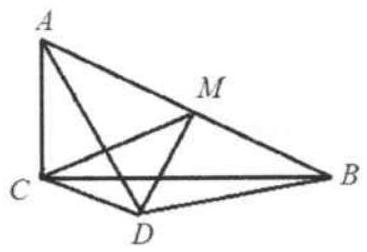
\includegraphics[width=\textwidth]{images/086.jpg} relatively prime, and \(n\) is not divisible by the square of any prime, find \(m+n+p\).

Solution: 578.
Draw \(C H \perp A B\) to meet \(A B\) at \(H\). Since \(D A=D B, D M\) is the perpendicular bisector of triangle \(D A B\). So \(D M \perp A B\).\\
Thus \(C H / / D M\). Connect \(D H\). We have\\
\(S_{\triangle C D M}=S_{\triangle H D M}=\frac{1}{2} H M \times D M\).\\
\(D M=\sqrt{A D^{2}-A M^{2}}=\frac{5 \sqrt{11}}{2}\),\\
\centering
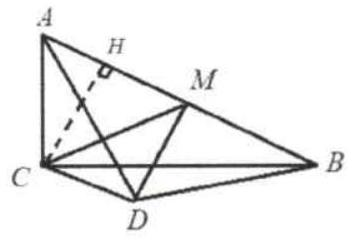
\includegraphics[width=\textwidth]{images/086(1).jpg}\\
\(H M=A M-A H=\frac{1}{2} A B-\frac{A C^{2}}{A B}=\frac{527}{50}\).\\
Thus \(C H / / D M\) and \(S_{\triangle C D M}=S_{\triangle H D M}=\frac{1}{2} H M \times D M=\frac{1}{2} \times \frac{5 \sqrt{11}}{2} \times \frac{527}{50}=\frac{527 \sqrt{11}}{40}\).\\
So \(m+n+p=527+11+40=578\).\\
\centering
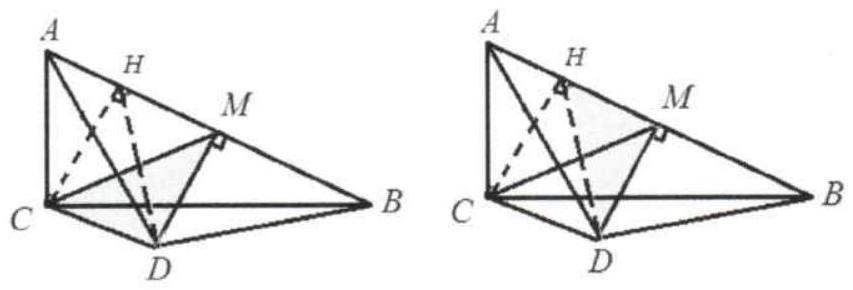
\includegraphics[width=\textwidth]{images/086(2).jpg}



\end{document}
